\subsection{Three Consecutive Fast Intervals}
\label{sec:tcfi}
\begin{figure}[t]
	\centering
	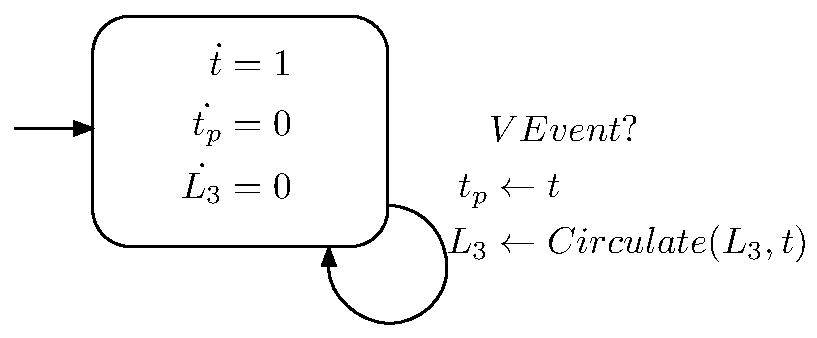
\includegraphics[scale=0.3]{figures/TCFI}
		\vspace{-10pt}
	\caption{Three Consecutive Fast Intervals $\Sys_{TCFI}$}
	\label{fig:tcfi}
\end{figure}
Our first module simply detects whether three consecutive fast intervals have occurred, where `fast' means the interval length, measured between 2 consecutive peaks on the \ac{EGM} signal, is shorter than some pre-set amount.
See Fig. \ref{fig:tcfi}.
States $t$ and $t_p$ are clocks as before.
The vector $L_3$ is three-dimensional, and stores the values of the last three intervals.
The event VEvent? is shorthand for the transition $y(t) \geq Th$ being taken by the $\Sys_{Sense}$ automaton.
In other words, it indicates a ventricular event.
Then $L_3$ gets reset to $L_3^+ = (z_1,z_2,z_3)^+ \defeq \text{Circulate}(L_3,t-t_p)$ where
\begin{equation}
L_3^+ = 
\left(\begin{matrix}
z_2\\z_3\\t-t_{p}\\
\end{matrix}
\right)
=
\left(\begin{matrix}
0 & 1 & 0\\0& 0& 1\\0& 0 &0
\end{matrix}
\right) L_3 + 
\left(\begin{matrix}
0\\0\\t-t_p
\end{matrix}
\right)
\end{equation}
%
\begin{lemma}
	$\Sys_{TCFI}$ is STORMED.
\end{lemma}
\begin{prf}
We show that the reset are monotonic - the other properties are easily checked.
For reset monotonicity, we invoke the fact that there is a minimum beat-to-beat separation: heartbeats can't follow one another with vanishingly small delays. 
In other words, there exists $m>0$ such that $t - t_p^- > m$.
Similarly, there's a maximum delay between two heartbeats, call it $B$.
Now, we seek a vector $\phi \in \Re^5$ s.t. 
\begin{equation}
\label{eq:tcfi resets}
\phi \cdot \left(\begin{matrix}
t-t\\t - t_p\\L_3^+ - L_3\\
\end{matrix}
\right) = \phi_p(t-t_p) +\phi_{L_3} \cdot \underbrace{\left(\begin{matrix}
z_2-z_1\\z_3-z_2\\t-t_p - z_3\\
\end{matrix}
\right)}_{\delta} \stackrel{Want}{\geq} \zeta > 0
\end{equation} 
Now $|\delta|$ is upper bounded by $\sqrt{3\cdot (2B)^2}$ since each element is the difference of intervals shorter than $B$.
Also, $t-t_p^- > m > 0$.
So choose $\phi_{L_3} = (\phi_{z,1},\phi_{z,2},\phi_{z,3})>0$ element-wise.
\eqref{eq:tcfi resets} is satisfied if the following stronger inequality is satisfied, which can be achieved by an appropriate choice of $\phi_{z,i}$: \;
$\phi_p m \geq \zeta + \sqrt{12B^2}\sum_1^3\phi_{z,i}$
\end{prf}

\subsection{Vector Timing Correlation}
\label{sec:VTC}
\begin{figure}[t]
	\centering
	\vspace{-15pt}
	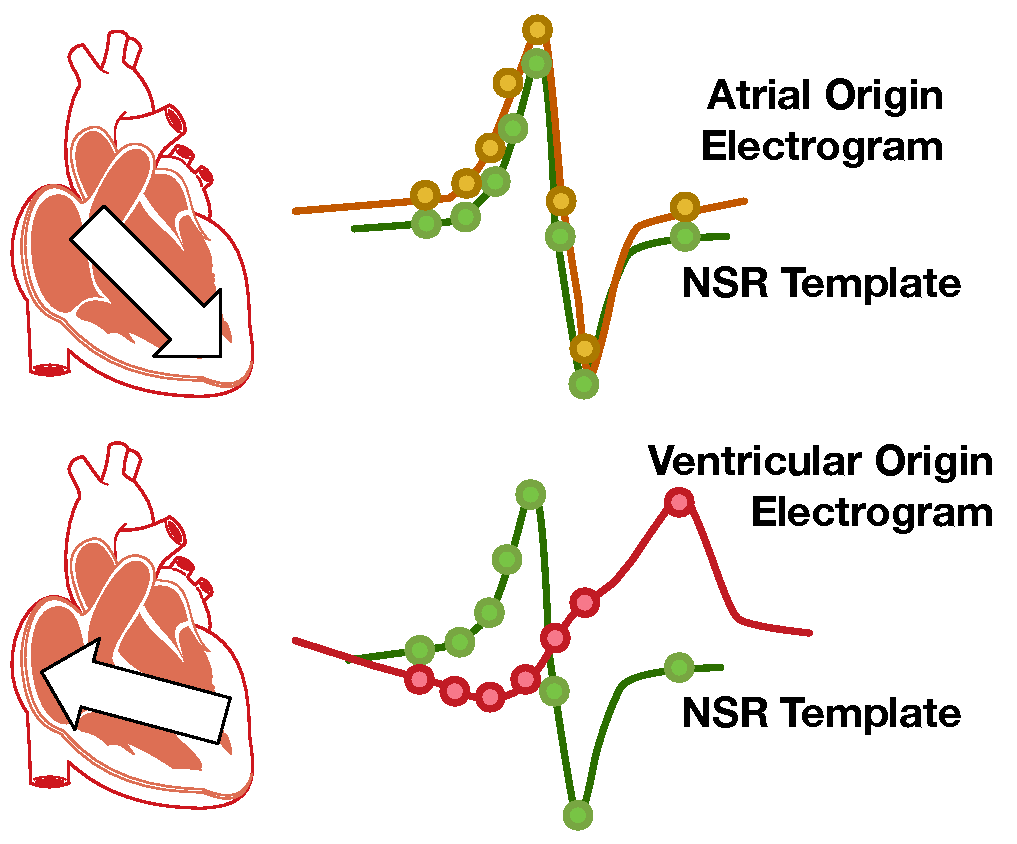
\includegraphics[scale=0.3]{figures/VTCEGMCompare}
	\caption{\small \acp{EGM} of different origin have different morphologies.}
	\label{fig:egmmorphology}
	\vspace{-10pt}
\end{figure}
%\caption{\small \acp{EGM} of different origin have different morphologies, while \acp{EGM} of same origin have very similar morphologies.}
It has been clinically observed that a depolarization wave originating in the ventricles (as produced during \ac{VT} for example) will in general produce a different \ac{EGM} morphology than a wave originating in the atria (as produced during \ac{SVT}) \cite{compass}.
See Fig. \ref{fig:egmmorphology}.
%
A morphology discriminator measures the correlation between the morphology of the current \ac{EGM} and that of a stored \emph{template} \ac{EGM} acquired during normal sinus rhythm.
If the correlation is above a pre-set threshold for a minimum number of beats, then this is an indication that the current arrhythmia is supraventricular in origin.
Otherwise, it might be of ventricular origin.

Boston Scientific's implementation of a morphology discriminator is called Vector and Timing Correlation (VTC).
VTC first samples 8 \emph{fiducial} points $\egm_i,i=1,\ldots,8$ on the current \ac{EGM} $\egm$ at pre-defined time instants.
Let $\egm_{m,i}$ be the corresponding points on the template \ac{EGM}.
A simple 0-shift correlation $\rho_{new}$ is calculated between the two sequences. 
If 3 out of the last 10 calculated correlation values exceed the threshold, then \ac{SVT} is decided and therapy is withheld.

The system of Fig. \ref{fig:HVTC} implements the VTC discriminator.
As before, $t$ is a local clock.
$\mu$ accumulates the values of the current \ac{EGM}, $\alpha$ accumulates the product $\egm_i \egm_{m,i}$, 
$\beta$ accumulates $\egm_i^2$.
State $w$ is an auxiliary state we need to establish the STORMED property.
$\vec{\nu}$ is a 10D binary vector: $\nu_i = -1$ if the $i^{th}$ correlation value fell below the threshold, and is $+1$ otherwise.
$L_3$ is the state of $\Sys_{TCFI}$: the guard condition $L_3 \leq th$ indicates that all its entries have values less than the tachycardia threshold, which is when $\Sys_{VTC}$ starts computing.
$WindowEnds$ indicates the `end' of an \ac{EGM}, measured as a window around the peak sensed by $\Sys_{Sense}$.  
%
\begin{figure}[t]
\centering
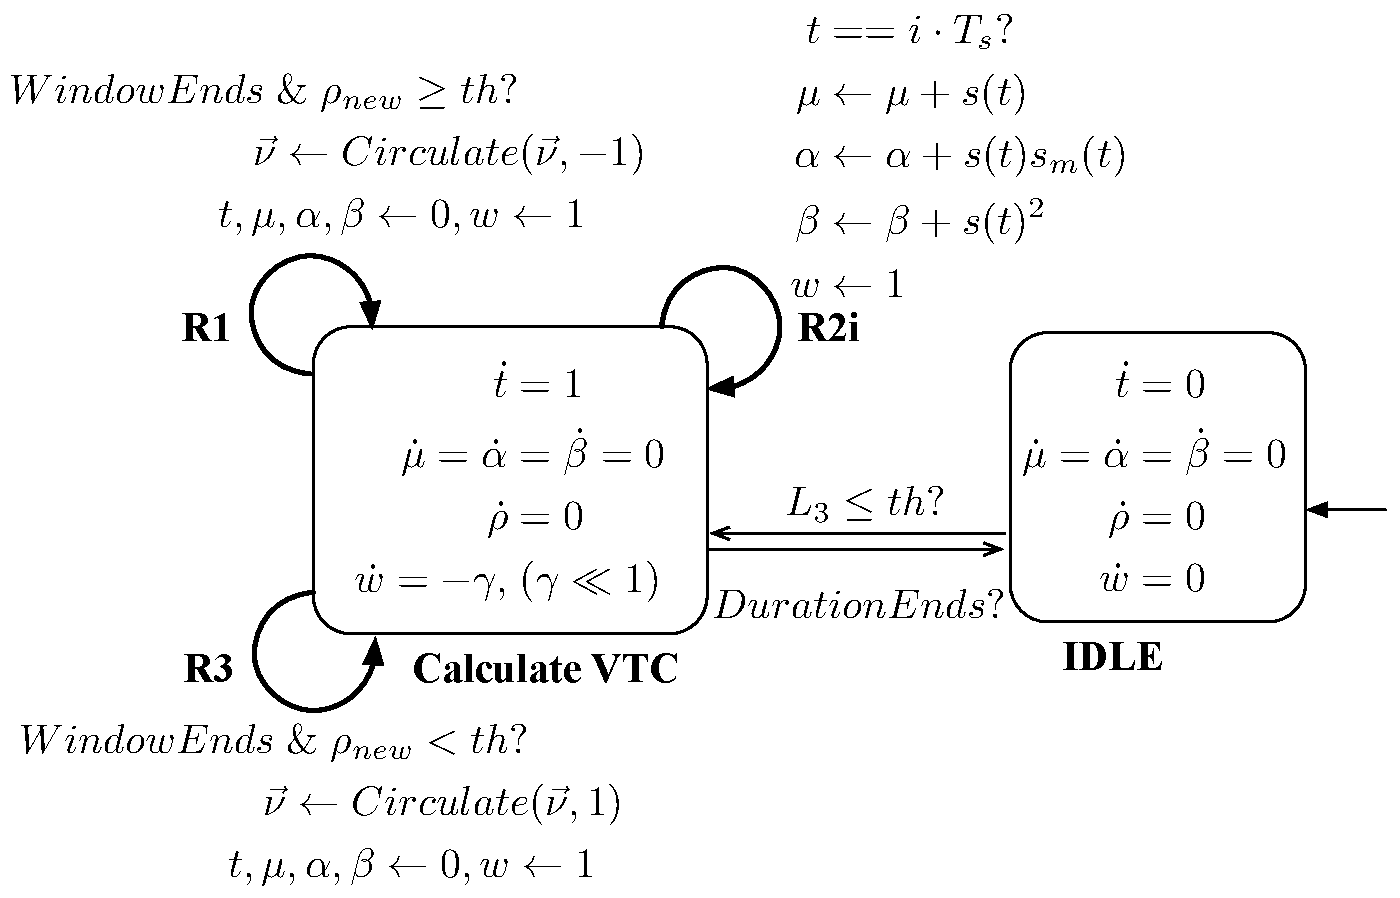
\includegraphics[scale=0.325]{figures/VTC1v2}
\vspace{-10pt}
\caption{VTC calculation. $iT_s$ is the sampling time for the $i${th} fiducial point, $i=1,\ldots,8$. $R2_{1},\ldots,R2_{8}$ are the corresponding resets. For clarity of the figure, 8 transitions are represented on the same edge.}
\vspace{-10pt}
\label{fig:HVTC}
\end{figure}
%
\begin{lemma}
	\label{lemma:vtc}
	$\Sys_{VTC}$ is STORMED.
	\end{lemma}

\subsection{Stability discrimination}
\label{sec:stability}
%\begin{figure}[t]
%	\centering
%	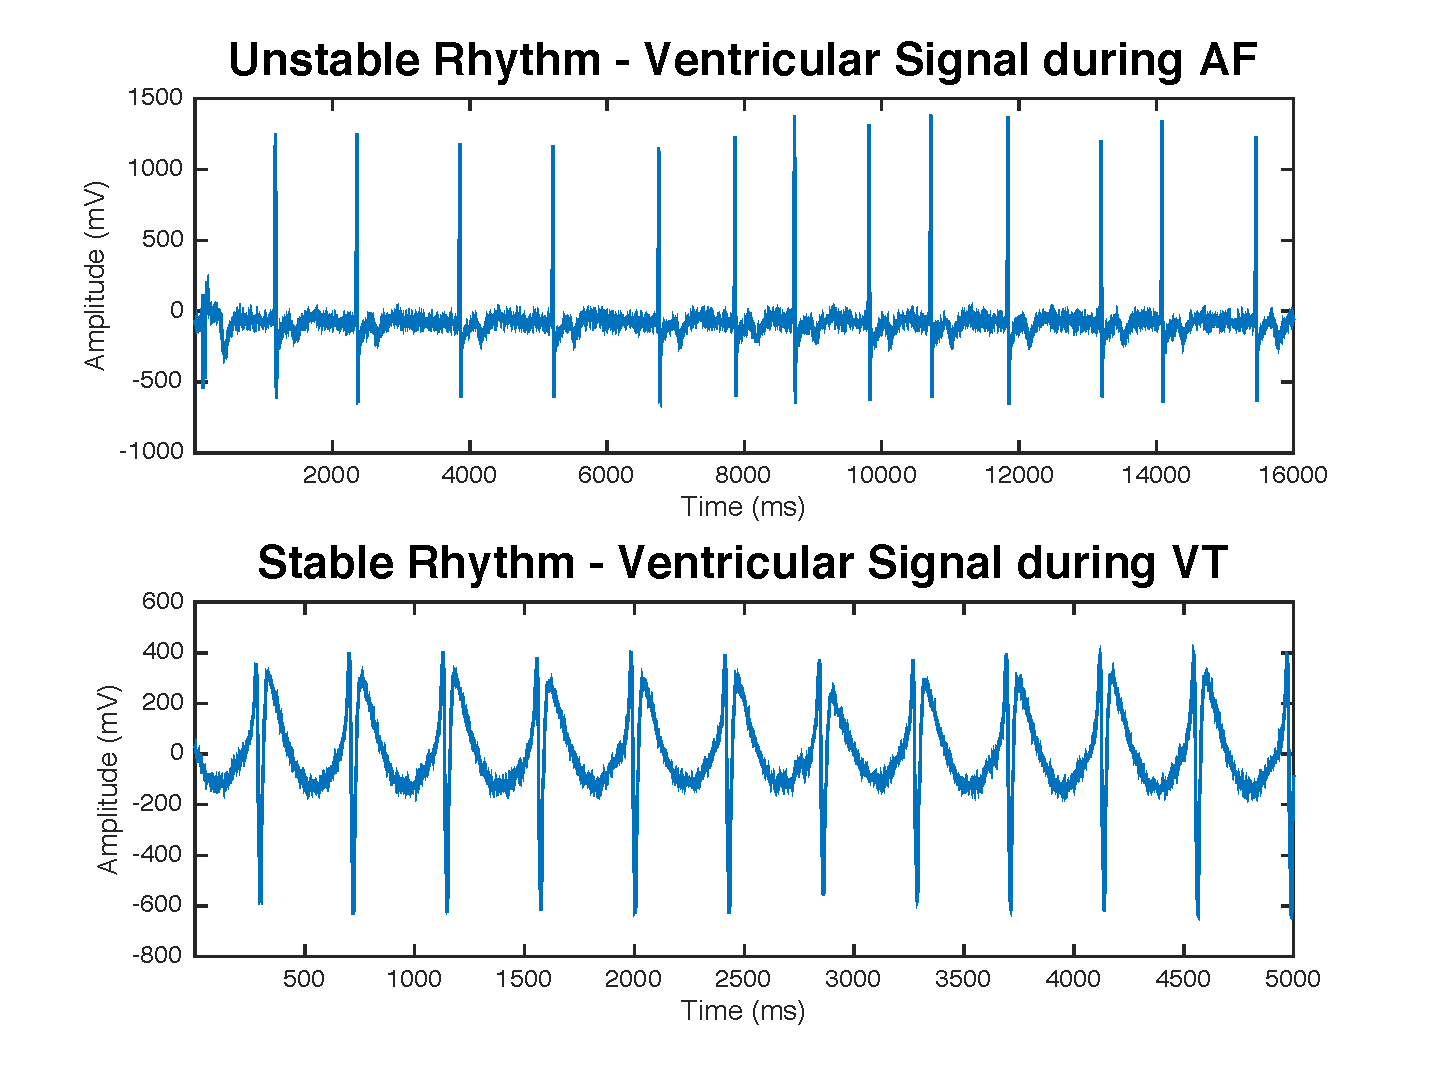
\includegraphics[scale=0.35]{figures/EGMStability}
%	\caption{Examples of a unstable rhythm (top) and stable rhythm (bottom).}
%	\label{fig:stable unstable}
%\end{figure}
\emph{Stability} refers to the variability of the peak-to-peak cycle length.
A rhythm with large variability (above a pre-defined threshold) is said to be \emph{unstable}, and is called stable otherwise.
The Stability discriminator is used to distinguish between atrial fibrillation, which is usually unstable, and \ac{VT}, which is usually stable.
%Atrial fibrillation, which is usually unstable, might induce a high ventricular rate .
%A \ac{VT}, on the other hand, is usually stable.
%Therefore this is a useful discriminator.

The Stability discriminator shown in Fig. \ref{fig:Hstab} simply calculates the variance of the cycle length over a fixed period called a Duration (measured in seconds).
Let $DL \geq 0$ be the Duration length.
The event $DurationEnds?$ indicates a transition of a simple system that measures the lapse of one Duration (not shown here).
State $t$ is a clock, $L_1$ accumulates the sum of interval lengths (and will be used to compute the average length), 
$L_2$ accumulates the squares of interval lengths,
and $\kappa$ is a counter that counts the number of accumulated beats.
$\sigma_2$ is assigned the value of the variance given by $\frac{1}{\kappa}[L_2 - 2L_1/\kappa + \kappa(L_1/\kappa)^2]$
\begin{figure}[t]
	\centering
	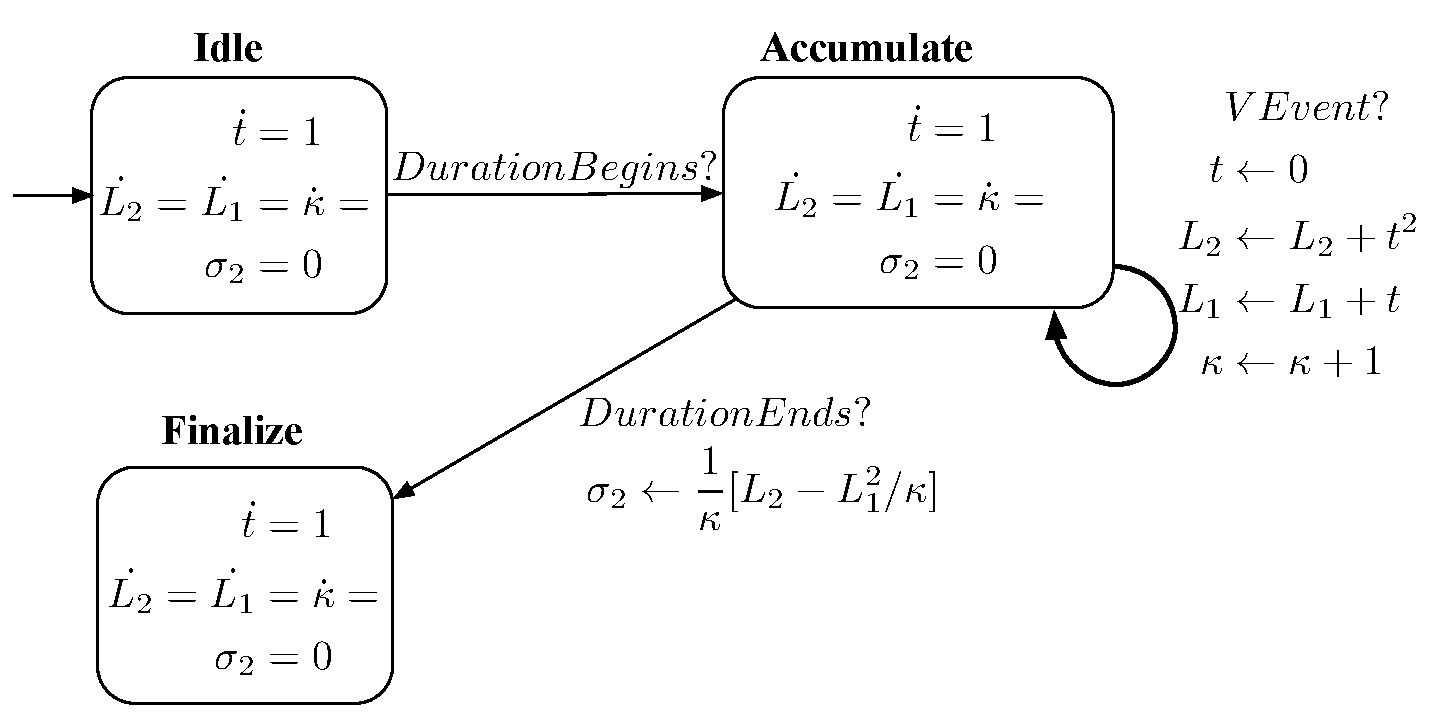
\includegraphics[scale=0.3]{figures/stability1v2}
	\vspace{-10pt}
	\caption{Stability discriminator.}
	\vspace{-10pt}
	\label{fig:Hstab}
\end{figure}

\begin{lemma}
	\label{lemma:stability}
	$\Sys_{Stab}$ is STORMED.	
\end{lemma}
The proof is in the Appendix.

Now that each system was shown to be STORMED, it remains to establish that their parallel composition is STORMED.
This result does not hold in general - Thm.~\ref{thm:SHS composition} gives conditions under which parallel composition respects the STORMED property.
Intuitively, we require that whenever a sub-collection of the systems jumps, the remaining systems that did not jump are separated from all of their respective guards by a uniform distance.
This is a requirement that can be shown to hold for our systems by modeling various minimal delays in the systems' operation. 
%For example, when a $VEvent?$ is issued by $\Sys_{Sense}$, $\Sys_{VTC}$ does not jump and will wait at least until the sampling time of the next fiducial point to make a transition.
%Or, when an atrial cell fires (in $\Sys_{CA}$), we model a minimal delay between it and all other cells that do not fire simultaneously.
We may now state:
\begin{thm}
Consider the collection of systems $\Sys_{CA}$, $\Sys_{ICD} = \Sys_{Sense} || \Sys_{Detection-Algo}$ where the latter is the parallel composition of the discriminator systems.
This collection satisfies the hypotheses of Thm. \ref{thm:SHS composition} (Section \ref{sec:compositionality}) and therefore the parallel system  $\Sys_{CA} || \Sys_{ICD}$ is STORMED and has a finite bisimulation.
\end{thm}


